\chapter{Ausgangslage und Zielstellung}\label{cha:Ausgangslage und Zielstellung}

Die in diesem Bericht dokumentierte Auslegung, beschäftigt sich mit dem Tragflügel des studentischen AUVSI Flugzeugs welches im Labor für Systemtechnik entwickelt wurde. Die vorangegangenen Flugzeuggenerationen und das Reglement der Wettbewerbs bilden die Ausgangslage für die Weiterentwicklung.

\section{Historie des AUVSI SUAS-Wettbewerbs}
Seit 2002 findet jährlich der AUVSI (Association for Unmanned Vehicle Systems International) SUAS (Student Unmanned Aerial Systems Competition)-Wettbewerb in den USA statt.

Hieran hat das studentische Hochschulteam in den Jahren 2015 und 2016 erfolgreich teilgenommen. Bereits im Jahr 2014 gab es die ersten Anstrengungen ein für diesen Wettbewerb passende Flugplattform zu entwickeln. Leider war dies zu diesem Zeitpunkt noch nicht von Erfolg gekrönt. Detaillierte Informationen hierzu können der Diplomarbeit von Herrn Dipl. Ing. Fabian Meilinger entnommen werden \cite{Meiling}.

Die meisten Anforderungen an die Flugplattform ergeben sich aus dem Reglement dieses studentischen Wettbewerbs. 

\clearpage

\section{Das Flugzeug des AUVSI SUAS Teams}

Seit den ersten Erfahrungen in der Saison 2014 folgt der Konzeptionelle Aufbau des Flugzeugs demselben stark modularen Konzept. Damit wurde mit klaren Schnittstellen zwischen den Baugruppen eine getrennte Weiterentwicklung der Einzelkomponenten möglich. Dadurch enstanden beispielsweise 2015 Variationen für die Forschungsmission im Regenwald Ecuadors bei der eine deutlich Voluminösere Nutzlast mitgeführt wurde \cite{Niclas}.

\begin{figure}[H]
\centering
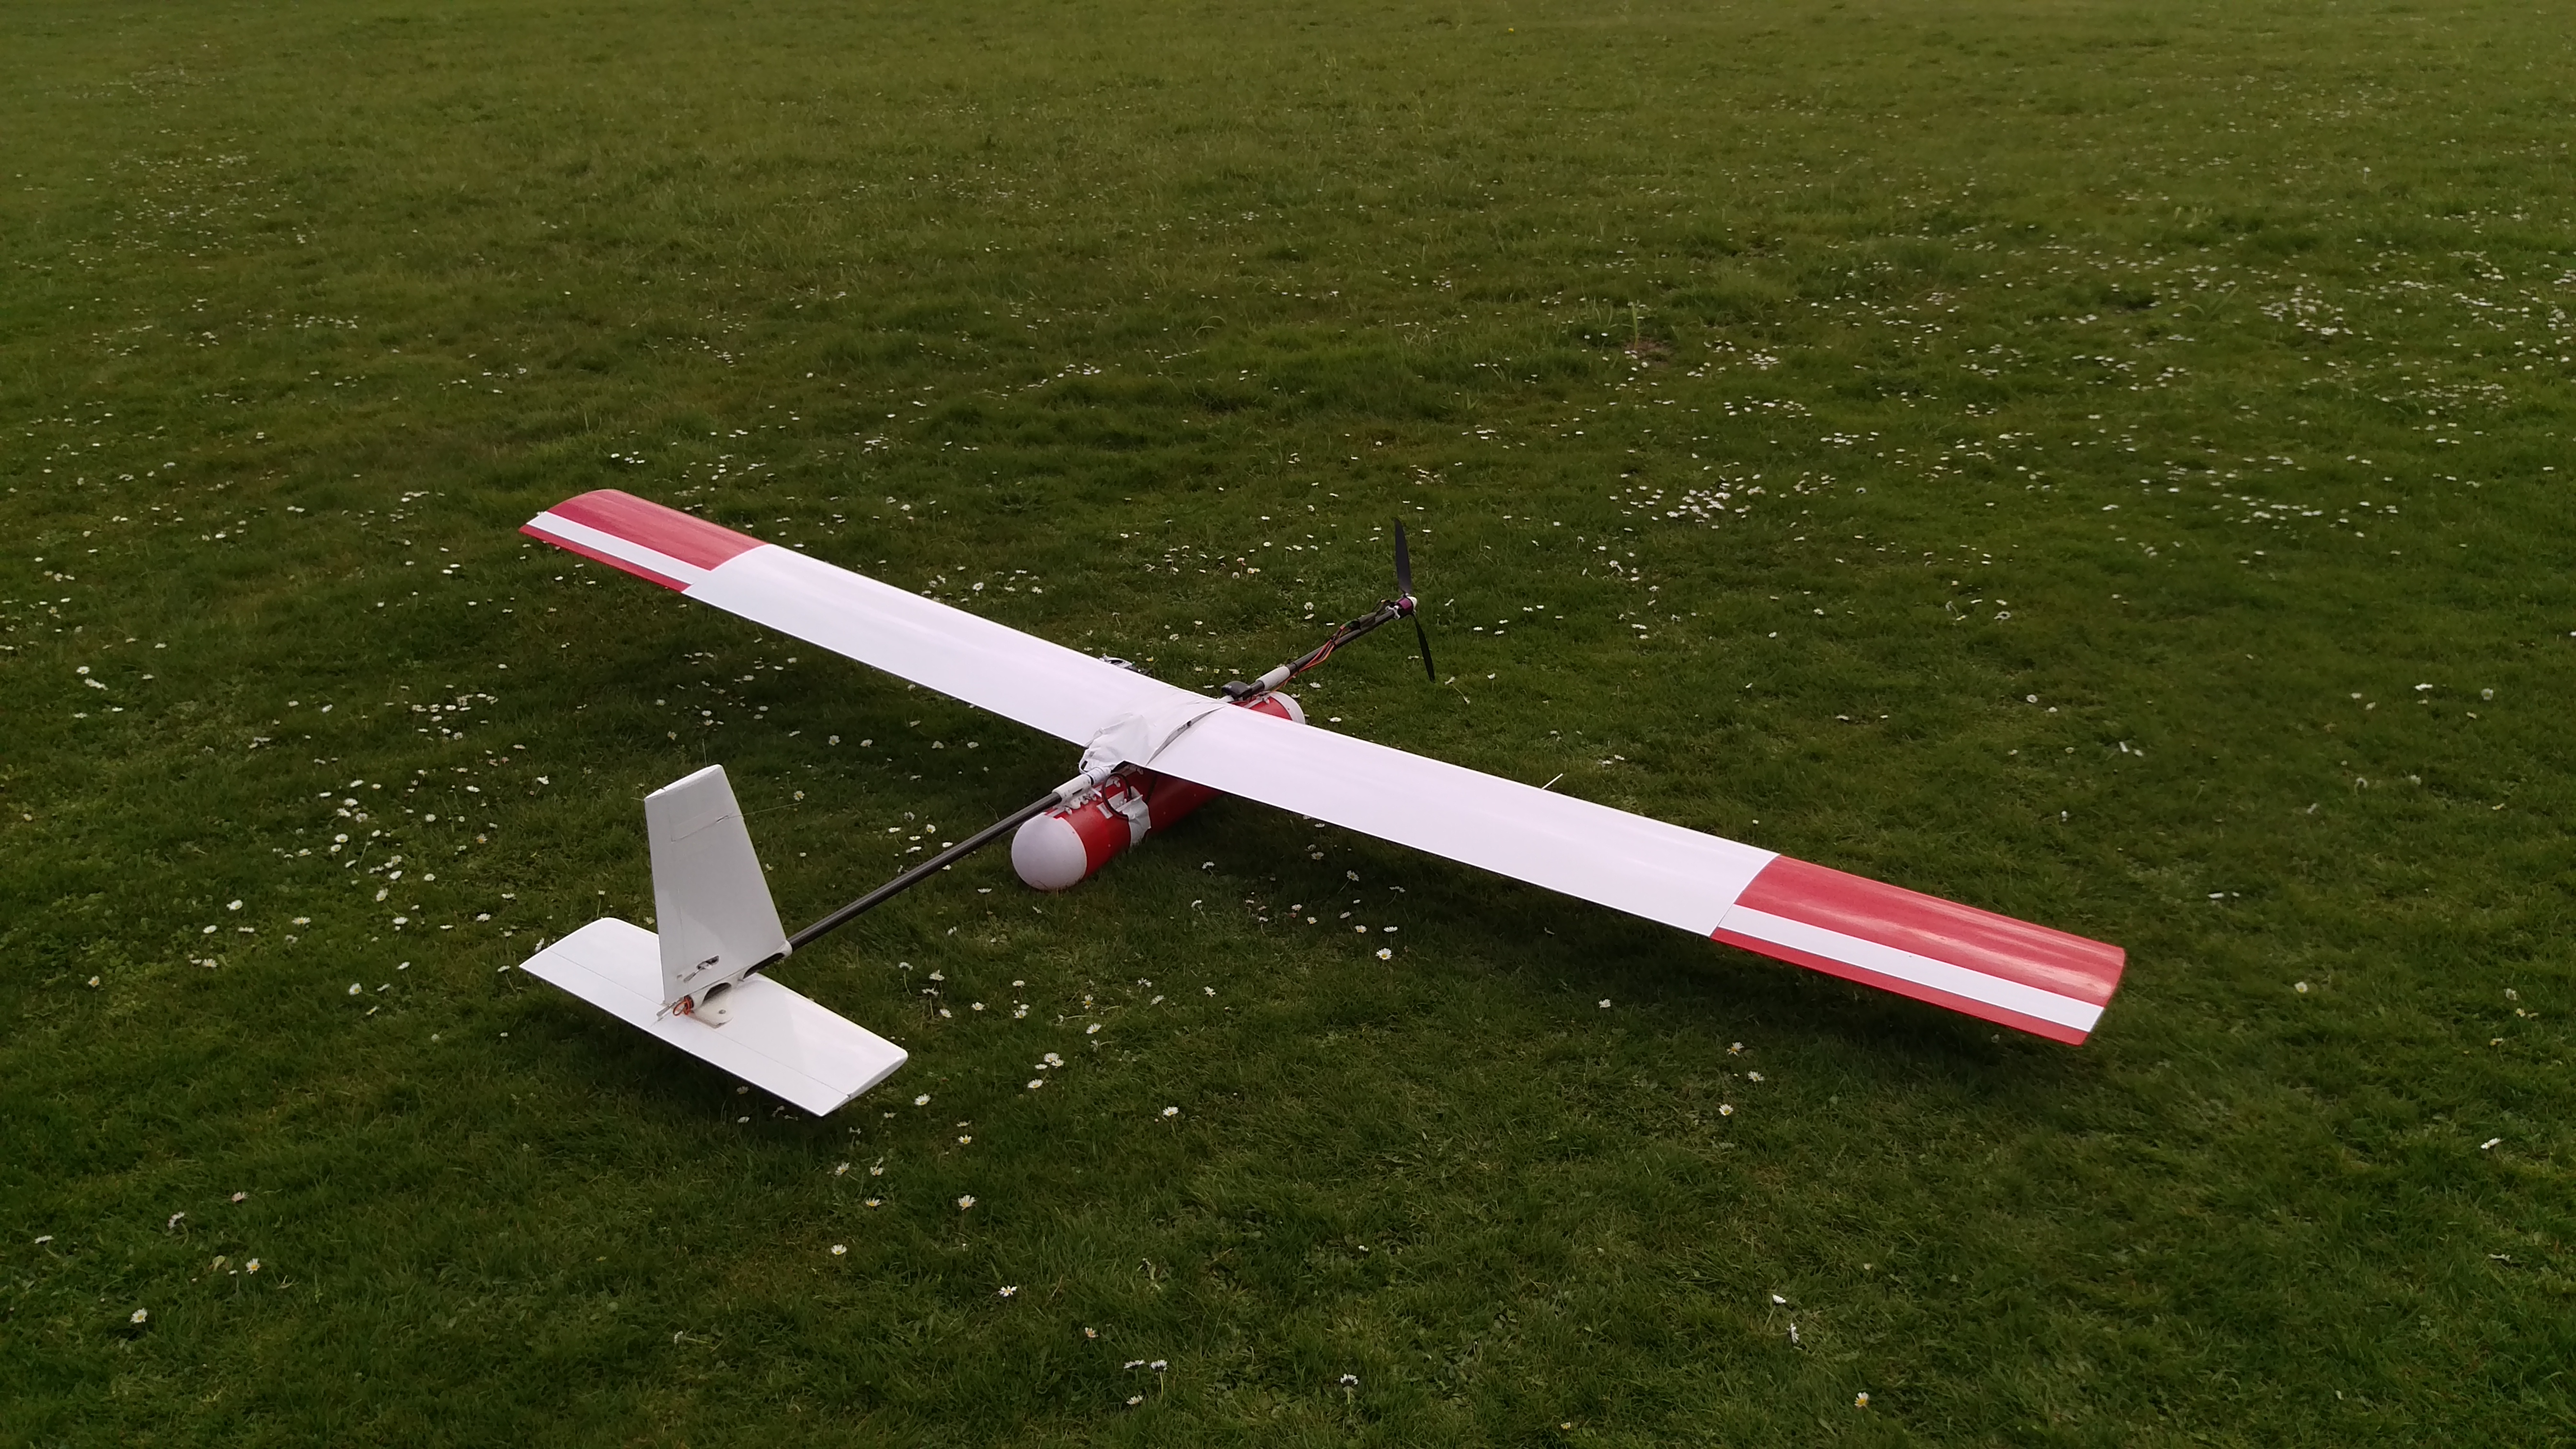
\includegraphics[width=0.9\textwidth]{bilder/Fotos/AUVSI_2015.jpg} 
\caption{Das AUVSI 2015 Modell im Einsatzzustand am Testflugplatz} 
\label{fig:Das AUVSI 2015 Modell in Einsatzzustand am Testflugplatz}
\end{figure}

Im Bild \ref{fig:Das AUVSI 2015 Modell in Einsatzzustand am Testflugplatz} ist der Gesamtaufbau des Flugzeugs zu sehen. Bisher sind der Einsatz von Rechteckigen Auftriebsflächen und Leitwerken sowie CFK-Rohren als Ausleger für Heck und Motorträger charakteristisch. Unter dem Zentralen Rumpfrohr ist der Zylinderförmige Nutzlastbehälter Montiert.

\section{Bisherige Flügelbauweise}


\section{Verbesserungsziele}

\section{Optimierungsgrenzen durch den Einsatz}